\section{Programming with QT}

\frame
{
\frametitle{What is QT?}
\begin{itemize}
\item Company History: Trolltech (1994-2008), Nokia (2008-2012), Digia (2012-2014), The QT Company (2014-)
\item QT is a cross-platform application and UI framework
\item QT provides intuitive C++ class libraries
\item Current Version: 5.12.0 (06-DEC-2018)
{\tiny
\begin{itemize}
\item 3D Graphics with OpenGL
\item Multithreading
\item Network Connectivity
\item Location and Positioning
\item ...
\end{itemize}
}
\item QT provides portability across several platforms\\
\begin{itemize}
\item Windows
\item OSX
\item Unix/Linux
\item Android
\item ...
\end{itemize}
\item QT provides development tools (IDE)
\end{itemize}
}

\subsection{QT Development Environment}
\frame
{
\frametitle{QT Development Environment}
Requirements
\begin{itemize}
\item MinGW
\item QT SDK
\item Editor: Notepad++, emacs, Ultra Edit, Atom, ...
\end{itemize}
\vspace{5mm}
Development Environment
\begin{itemize}
\item Console
\item QT Creator
\item Visual Studio, Code Blocks, ... (not supported@hf-ict)
\end{itemize}
}

\frame
{
\frametitle{Development with Console}
\begin{itemize}
\item Change to the directory containing the source code
\item Type \emph{qmake -project [CONFIG+=console]}
\item Type \emph{qmake}
\item Type \emph{mingw32-make}
\end{itemize}

Ensure that the correct Environment variables are set (PATH)!\\
\begin{itemize}
\item QT bin folder
\item MINGW bin folder
\end{itemize}
}

\frame
{
\frametitle{Development with QT Creator}
\begin{itemize}
\item Start the QT Creator application
\item File - New - QT 5 Gui Application
\item Enter project name
\item Select required modules
\item Start the application with Build - Run
\end{itemize}
}

\frame
{
\frametitle{Development with QT Creator}
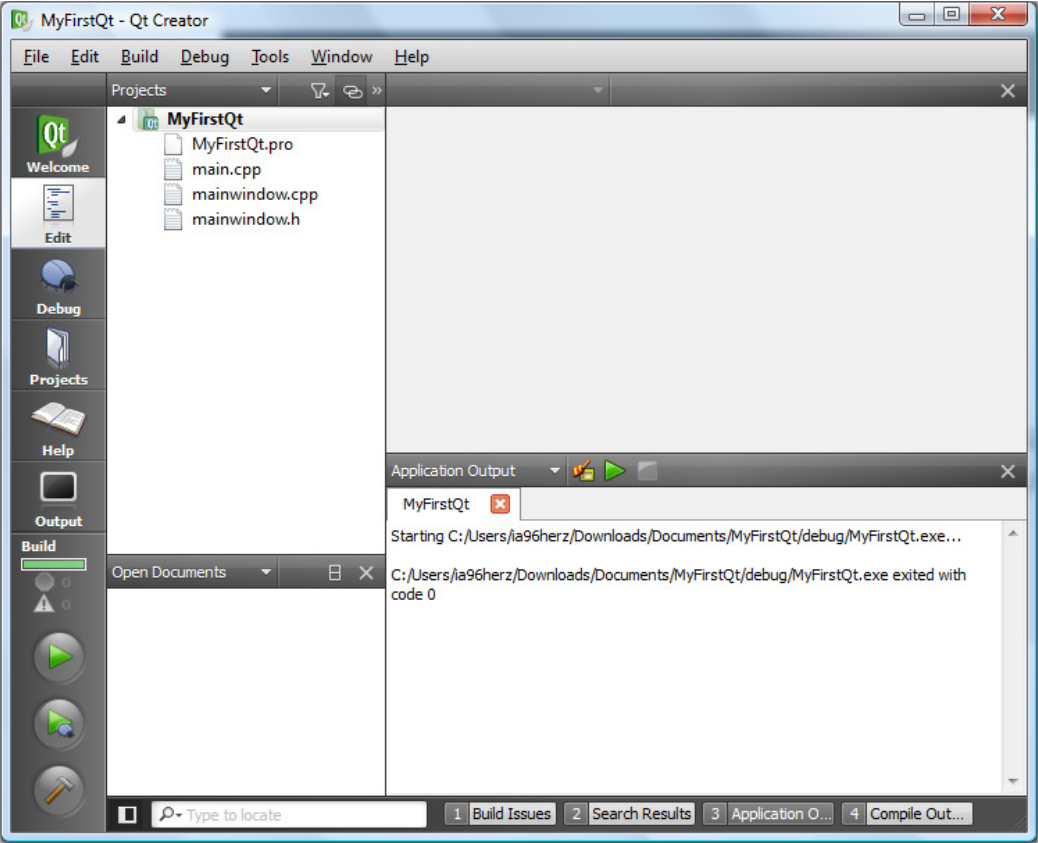
\includegraphics[width=250pt]{img/qtcreator.png}
}

\frame
{
\frametitle{Resources}
The complete Documentation, API and Examples can be found at
\begin{itemize}
\item https://doc.qt.io
\end{itemize}
Books:
\begin{itemize}
\item Mastering Qt 5\\
Guillaume Lazar, Robin Penea\\
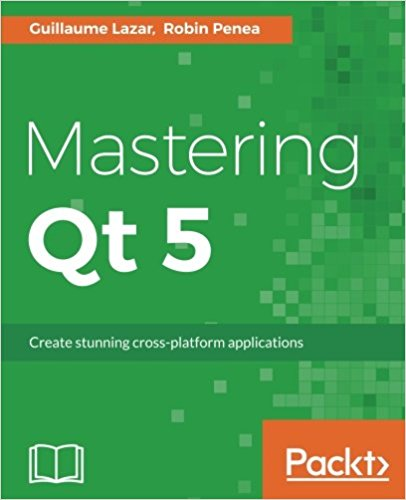
\includegraphics[width=90pt]{img/qt5book.jpg}
\end{itemize}
}

\frame
{
\frametitle{QT - HF-ICT}
\begin{itemize}
\item Introduction
\item Small Projects (QT Basics, Layouts, Slots, ...)
\item Fractals (QT Painting)
\item Game (Multithreading)
\end{itemize}
}

\subsection{Hello World - Hello QT - Basics}
\frame
{
\frametitle{Hello QT - My first QT program}
\lstinputlisting{code/qt/helloqt/helloqt.cpp}
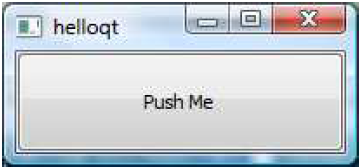
\includegraphics[width=85pt]{img/helloqt.png}
}

\frame
{
\frametitle{Exercise - Hello QT}
\begin{exercise}
\begin{itemize}
\item Setup your QT development environment
\item Write a \emph{Hello QT} application
\end{itemize}
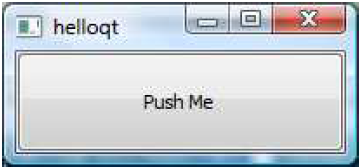
\includegraphics[width=85pt]{img/helloqt.png}
\end{exercise}
}

\begin{frame}[fragile]
\frametitle{QWidget}
Every gui element (single element or a group of element) in QT is a Widget (Window Gadget).
\vspace{5mm}
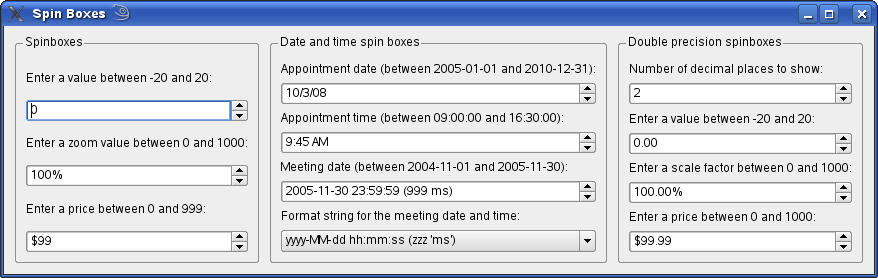
\includegraphics[width=280pt]{img/widget.png}
\end{frame}

\begin{frame}[fragile]
\frametitle{Exercise - QT Standard Widgets}
\begin{exercise}
Create the following three QT applications:\\
\vspace{5mm}
\\
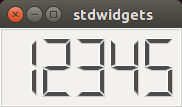
\includegraphics[width=75pt]{code/qt/stdwidgets/w1.png}
\hspace{5mm}
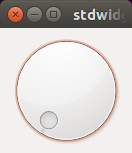
\includegraphics[width=50pt]{code/qt/stdwidgets/w2.png}
\hspace{5mm}

\includegraphics[width=100pt]{code/qt/stdwidgets/w3.png}
\end{exercise}
\end{frame}

\begin{frame}[fragile]
\frametitle{Exercise - 2 Widgets in one Window}
\begin{exercise}
Can you display two widgets in one window?\\
\vspace{5mm}
\\
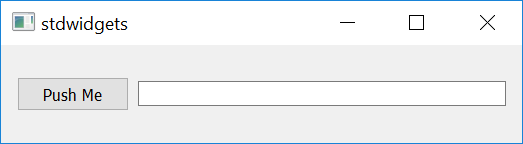
\includegraphics[width=120pt]{code/qt/stdwidgets/w4.png}
\end{exercise}
\end{frame}


\begin{frame}[fragile]
\frametitle{QDebug vs cout}
\begin{itemize}
\item qDebug()
\item qInfo()
\item qWarning()
\item qCritical()
\item qFatal()
\end{itemize}

\begin{lstlisting}
qDebug() << "some debug output...";
\end{lstlisting}

Switch off debug output:
\begin{lstlisting}
qmake -project DEFINES+=QT_NO_DEBUG_OUTPUT
\end{lstlisting}

\end{frame}


\subsection{Layout Manager}
\frame
{
\frametitle{Layout Manager}
The following Layout Managers are available in QT:
\begin{itemize}
\item QHBoxLayout
\item QVBoxLayout
\item QGridLayout
\item QFormLayout
\item Null Layout
\item ...
\end{itemize}
}

\begin{frame}[fragile]
\frametitle{QHBoxLayout (QVBoxLayout)}
Horizontal arrangement of all widgets.\\
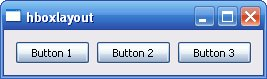
\includegraphics[width=112pt]{code/qt/hbox/hboxlayout.jpg}\\
{\tiny
\lstinputlisting{code/qt/hbox/hbox.cpp}
}
\end{frame}

\begin{frame}[fragile]
\frametitle{QHBoxLayout (QVBoxLayout)}
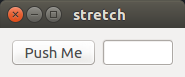
\includegraphics[width=100pt]{code/qt/stretch/stretch1.png}\\
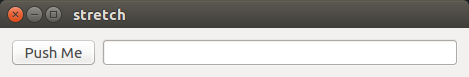
\includegraphics[width=150pt]{code/qt/stretch/stretch2.png}\\
\begin{lstlisting}
button->sizePolicy().expandingDirections();
// QFlags()
input->sizePolicy().expandingDirections();
// QFlags(0x1)
// 0x1: Qt::Horizontal
\end{lstlisting}
\end{frame}

\frame
{
\frametitle{QGridLayout}
Arrangement of all widgets in a grid.\\
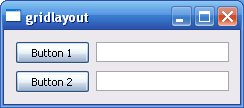
\includegraphics[width=100pt]{code/qt/grid/gridlayout.jpg}\\
{\tiny
\lstinputlisting{code/qt/grid/gridlayout.cpp}
}
}

\frame
{
\frametitle{QFormLayout}
The QFormLayout class manages forms of input widgets and their associated labels.\\
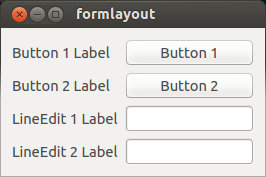
\includegraphics[width=100pt]{img/formlayout.png}\\
{\tiny
\lstinputlisting{code/qt/formlayout/mywidget.cpp}
}
}

\frame
{
\frametitle{Null Layout}
No layout manager\\
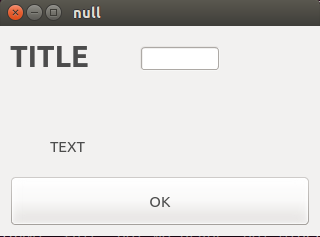
\includegraphics[width=72pt]{code/qt/null/xylayout.png}\\
{\tiny
\lstinputlisting{code/qt/null/mywidget.cpp}
}
}

\begin{frame}[fragile]
\frametitle{Modular Programming}
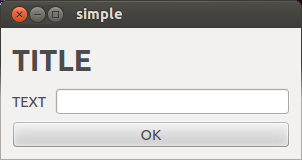
\includegraphics[width=140pt]{img/simple.png}
\hspace{4mm}
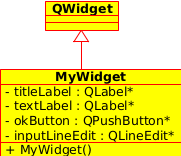
\includegraphics[width=100pt]{img/simplecd.png}
\end{frame}

\begin{frame}[fragile]
\frametitle{Modular Programming}
{\tiny
\lstinputlisting{code/qt/simple/mywidget.h}
}
\end{frame}

\begin{frame}[fragile]
\frametitle{Modular Programming}
{\tiny
\lstinputlisting{code/qt/simple/mywidget.cpp}
}
\end{frame}

\begin{frame}[fragile]
	\frametitle{Modular Programming}
	{\tiny
	\lstinputlisting{code/qt/simple/main.cpp}
	}
\end{frame}

\frame
{
	\frametitle{QMainWindow}
	A main window provides a framework for building an application's user interface.
	Qt has QMainWindow and its related classes for main window management.
	QMainWindow has its own layout to which you can add QToolBars, QDockWidgets,
	a QMenuBar, and a QStatusBar. The layout has a center area that can be occupied
	by any kind of widget.\\
	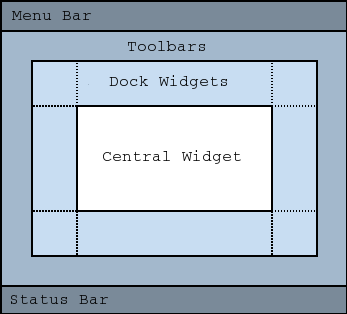
\includegraphics[width=140pt]{img/mainwindowlayout.png}

}

\frame
{
	\frametitle{Change Background Color of QLineEdit}
	\lstinputlisting{code/qt/color.cpp}
}

\frame
{
	\frametitle{Validate Input}
	There are two ways on how to validate the input values.
	\begin{itemize}
	\item Using a validator
	{\tiny
	\lstinputlisting{code/qt/validator/method1.cpp}
	}
	\item Check the values after commit
	{\tiny
	\lstinputlisting{code/qt/validator/method2.cpp}
	}
	\end{itemize}
}


\subsection{Event Handling}
\frame
{
	\frametitle{Slots}
	Every widget may fire events (Signals). These events can be catched be a method
	called slot.\\
	Take a look on the API to check which Signal and Slots are available for each
	widget.\\
	Example: Signals of the class QPushButton:
	\begin{itemize}
	\item clicked(bool checked=false)
	\item pressed()
	\item released()
	\item toggled(bool checked)
	\end{itemize}
}

\frame
{
	\frametitle{Slots}
	A class which implements a slot must
	\begin{itemize}
	\item be inherited from the class QObject (or a subclass)
	\item contain the Q\textunderscore OBJECT statement
	\item contain the public slots section
	\end{itemize}
	\lstinputlisting{code/qt/slot.cpp}
}

\frame
{
	\frametitle{Slots}
	Within the code, the Signal and Slot must be connected.
	\lstinputlisting{code/qt/connection.cpp}
	The senderObject fires the event (signal). The receiverObject contains the slot.
}

\begin{frame}[fragile]
	\frametitle{My first slot}
	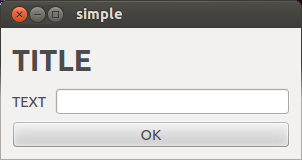
\includegraphics[width=140pt]{img/simple.png}
	\hspace{4mm}
	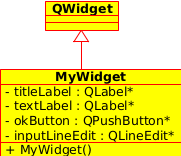
\includegraphics[width=100pt]{img/simplecd.png}\\
	\vspace{3mm}
	Add a simple slot called \verb|onButtonClicked| in the class \verb|MyWidget|.
\end{frame}

\begin{frame}[fragile]
	\frametitle{My first slot}
	\begin{lstlisting}
class MyWidget : public QWidget {
Q_OBJECT
private:
  ... // see slide before
public:
  ... // see slide before
public slots:
  void onButtonClicked();
	\end{lstlisting}
\end{frame}

\begin{frame}[fragile]
	\frametitle{My first slot}
	\begin{lstlisting}
MyWidget::MyWidget() {
  ... // see slide before
  QOBject::connect(
    okButton, SIGNAL(clicked()),
    this, SLOT(onButtonClicked()));
}

void MyWidget::onButtonClicked() {
  // delete the content of the QLineEdit component
  inputLineEdit->clear();
}
	\end{lstlisting}
\end{frame}

\begin{frame}[fragile]
	\frametitle{Exercise - Event Handling}
	Take the code from the example above. Add a new class called \verb|EventHandler|
	and move the slot \verb|onButtonClicked| from the class \verb|MyWidget| to the
	class \verb|EventHandler|. The functionality should still be the same.
\end{frame}

\begin{frame}[fragile]
	\frametitle{Exercise - Event Handling}
	The major difficulties in this exercise are:
	\begin{itemize}
	\item A new object of the class \verb|EventHandler| must be created and used
	within the \verb|QObject::connect| statement.
	\item A way must be found to access the \verb|inputLineEdit| component, which
	is now in another class than the slot.
	\end{itemize}
\end{frame}

\begin{frame}[fragile]
\frametitle{Signals}
Every widget may fire events (Signals). A signal will be implemented
in the following way:

{\small
\begin{lstlisting}
class MyClass : public QObject {
public:
  MyClass();
  ...
  void someMethod();
signals:
  void somethingHappens();
};
\end{lstlisting}
}
A signal method has no implementation. The signal itself can be
triggered by calling the method:

{\small
\begin{lstlisting}
void MyClass::someMethod() {
   emit somethingHappens();
}
\end{lstlisting}
}

\end{frame}

\subsection{Dialogs}
\begin{frame}[fragile]
\frametitle{Dialogs}
In a graphical user interface, a dialog is a window used to enable communication between
a computer and the user. It may communicate information to the user, prompt the user for
a response, or both. A dialog can be displayed in modal mode.\\
\vspace{3mm}
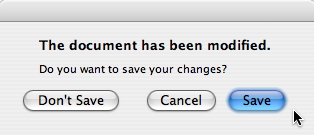
\includegraphics[width=160pt]{img/dialog1.png} 
\end{frame}

\begin{frame}[fragile]
\frametitle{Dialogs}
The class QMessageBox could be used fo standard dialogs:
\vspace{3mm}
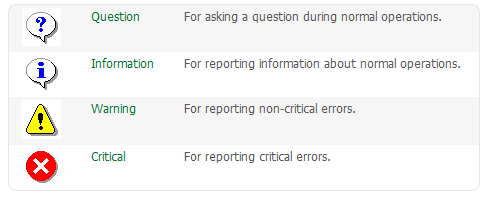
\includegraphics[width=200pt]{img/messagebox.png}
{\tiny
\begin{lstlisting}
int result = QMessageBox::warning( // warning, critical, ...
  this, // parent
  "TITLE",
  "TEXT",
  QMessageBox::Save | QMessageBox::Discard | QMessageBox::Cancel
);
\end{lstlisting}
}
\end{frame}

\begin{frame}[fragile]
\frametitle{Dialogs}
If a custom dialog is needed, create a class inherited from QDialog.
A dialog is created like a QWidget (actually it is a QWidget) with
some additional important dialog functionality.
\begin{itemize}
\item Modal - Calling window is disabled and the dialog is always in foreground.
\item Result - A dialog normally provides a result value.
(e.g. Ok, Cancel Button Clicked)
\end{itemize}
\end{frame}

\begin{frame}[fragile]
	\frametitle{Exercise - Modular Programming}
	\begin{exercise}
  Implement a gui to validate a credit card number (only the number).\\
  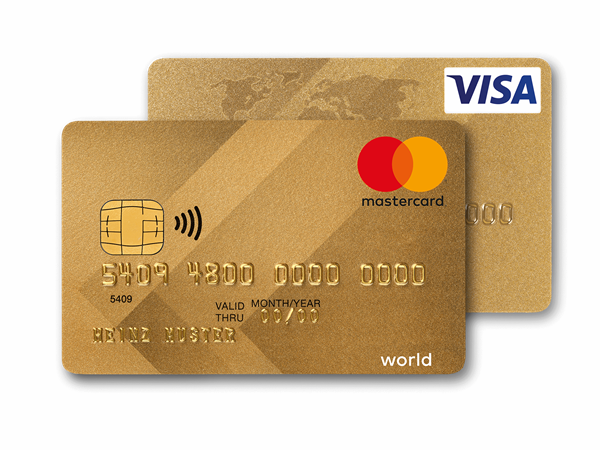
\includegraphics[width=140pt]{img/creditcard.png}\\
  The Luhn formula can be used to validate the number.
	\end{exercise}
\end{frame}


\subsection{Painting}
\begin{frame}[fragile]
\frametitle{Painting}
To paint something on a QT Widget, the method paintEvent must be overwritten:
\lstinputlisting{code/qt/paint/paint.cpp}
\end{frame}

\begin{frame}[fragile]
\frametitle{Painting}
The QPainter objects supports many method to draw specific geometric figures:
	(e.g. Arc, Line, Point)\\
	\vspace{3mm}
        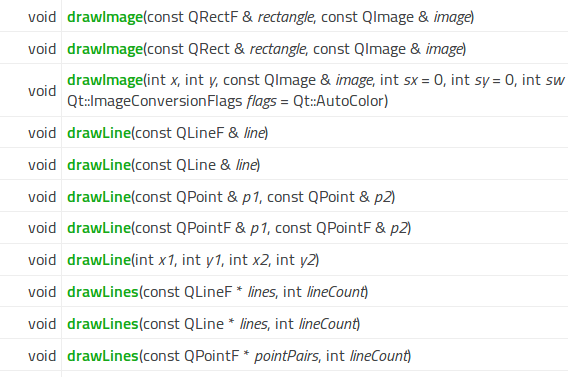
\includegraphics[width=190pt]{img/painter.png}
\end{frame}

\begin{frame}[fragile]
\frametitle{Exercise - Moiree}
Create an application which draws the following picture:\\
\vspace{3mm}
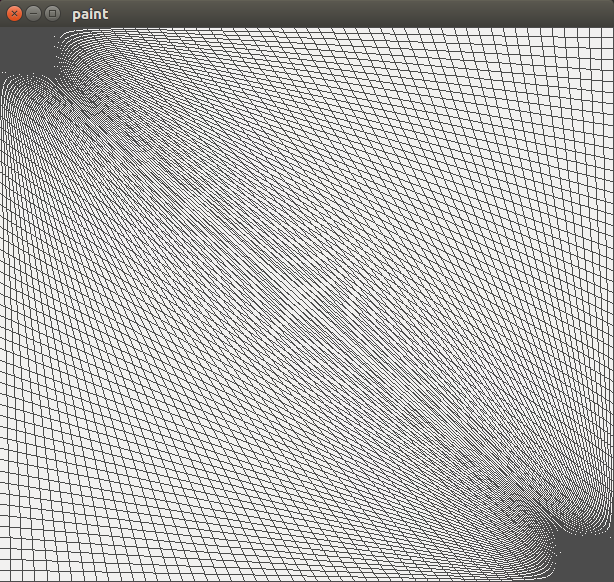
\includegraphics[width=190pt]{img/moiree.png}
\end{frame}

\begin{frame}[fragile]
\frametitle{Exercise - Sierpinski}
Draw on a widget with the following algorithm:
{\small
\begin{enumerate}
\item Create 3 random points A, B and C. Preferably the 3 points should
be a triangle stretched over the widget.
\item Define a point (x,y) which is equal to point A.
\item Define randomly a point A, B or C. This point is called Z.
\item Calculate the middlepoint ($x_m$ and $y_m$) between Z and (x, y).
\item Draw a point at position $x_m$ and $y_m$.
\item Set $x=x_m$ and $y=y_m$.
\item o to step 3
\end{enumerate}
}
\end{frame}

\begin{frame}[fragile]
\frametitle{Exercise - Mandelbrot Set}
Create an application which draws the following picture:\\
\vspace{3mm}
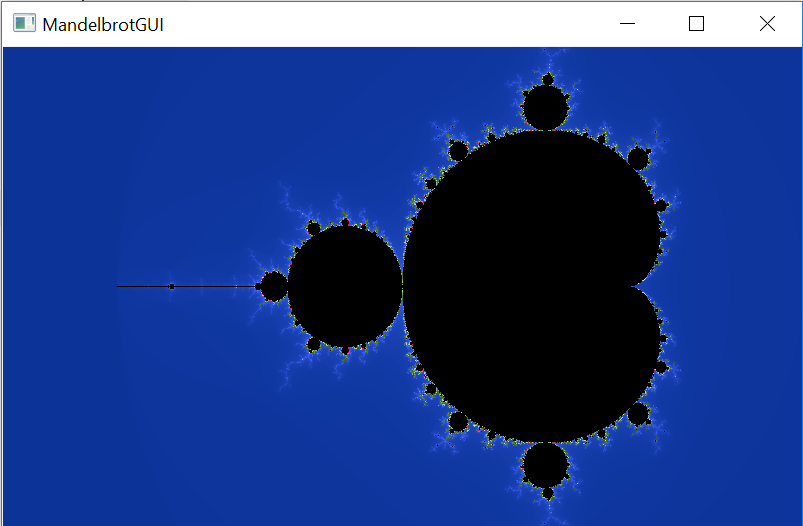
\includegraphics[width=220pt]{img/Mandelbrot.png}
\end{frame}

\begin{frame}[fragile]
\frametitle{Exercise - Mandelbrot Set}
Create a widget named `'Mandelbrot'' that implements the following algorithm:
{\small
\begin{enumerate}
\item Set the minimum Size of the Widget to x=800, y=480
\item Overload the paintEvent method and iterate over all pixels of the widget. 
\item Implement a method calcMandelbrotPoint that accepts the x-coordinate (int Px) and y-coordinate (int Py) and a recusrsion limit (int maxIterations=200)
	\begin{itemize}
	\item Scale the coordinate Px linear to the numeric range from -2.5 to 1.0 (Save the scaled value in x1)
	\item Scale the coordinate Py linear to the numeric range from -1.0 to 1.0 (Save the scaled value in y1)
	\item Initialize double x0 = 0.0 and y0 = 0.0
	\item Loop as long ${x_0}^2 \cdot {y_0}^2 < 4.0$ and as long the iteration counter is not exceeding maxIterations.
	\item Calculate Real Number $x_0 = {x_0}^2 - {y_0}^2 + x_1$ (only replace the x0 variable value after the next operation)
	\item Calculate Imaginary Number $y_0 = 2 \cdot  x_0 \cdot y_0  \cdot + y_1$ 
	\item Increase Iteration counter on each loop - return the amount of iterations performed
	\end{itemize}
\item Evaluate if the returned Iteration Counter of calcMandelbrotPoint - if the counter is greater than 100 set a black point. Optionally define a gradient palette of various colors for a range 0..n.
\end{enumerate}
}
\end{frame}

\subsection{Mouse Events}
\begin{frame}[fragile]
\frametitle{Mouse Events}
Mouse move and and mouse click events can be tracked on a widget by
overwritting one (or both) of the following methods:

\begin{itemize}
\item \verb|mouseMoveEvent(QMouseEvent *event)|\\
Do not forget to switch on mouse tracking (\verb|setMouseTracking(true)|) to handle these events.
\item \verb|mousePressEvent(QMouseEvent *event)|
\item \verb|mouseDoubleClickEvent(QMouseEvent *event)|
\item \verb|mouseReleaseEvent(QMouseEvent *event)|
\end{itemize}

\end{frame}

\subsection{Threads}
\begin{frame}[fragile]
\frametitle{Threads}
A Thread in QT may be implemented in the following way:
{\tiny
\begin{lstlisting}
class MyThread : public QThread {
public:
  void run();
};

void MyThread::run() {
  // code which will be executed in the thread
}

// creating a thread
MyThread *mt = new MyThread();
// starting a thread
mt.start();
\end{lstlisting}
}
\end{frame}

\begin{frame}[fragile]
\frametitle{Threads}
Endless Thread with the possibility to stop.
{\tiny
\begin{lstlisting}
class MyThread : public QThread {
private:
  bool running;
public:
  MyThread();
  void stopThread();
  void run();
};

MyThread::MyThread() : running(true) {}

void MyThread::stopThread() {
  running = false;
}

void MyThread::run() {
  while(running) {
  // code which will be executed in the thread
  msleep(50);
  }
}
\end{lstlisting}
}
\end{frame}

\begin{frame}[fragile]
\frametitle{Threads}
Thread Synchronization - Producer Consumer\\
{\tiny
The Producer-Consumer problem describes two processes, the producer and the consumer, who share a data container. The producer's job is to generate data. The consumer's job is to consume (and remove) the data. The problem is to make sure that the producer won't try to add data into the container if it's full and that the consumer won't try to consume data from an empty container.
}
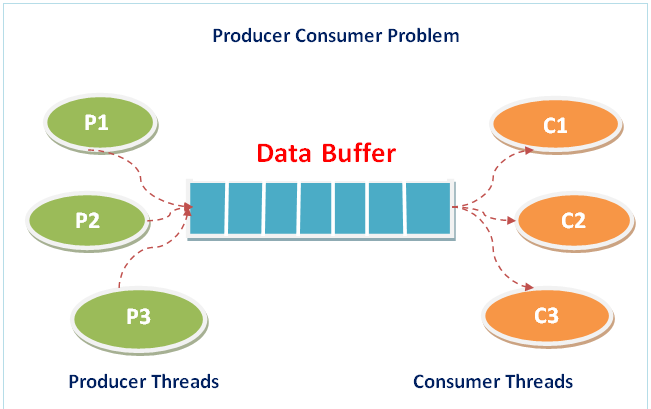
\includegraphics[width=190pt]{img/prodcon.png}

\end{frame}

\begin{frame}[fragile]
\frametitle{Threads}
Thread Synchronization - Producer Consumer\\
QT provides several classes for thread synchronization:
\begin{itemize}
\item QMutex
\item QSemaphore
\item QMutexLocker
\item QWaitConditon
\item QReadWriteLock
\end{itemize}

\end{frame}

\begin{frame}[fragile]
\frametitle{Threads}
Thread Synchronization - Producer Consumer\\
{\tiny
\lstinputlisting{code/qt/thread/prodcon.cpp}
}

\end{frame}

\begin{frame}[fragile]
\frametitle{QT Game}
The following slides will describe how to create a simple game in QT.
\begin{itemize}
\item Idea
\item Gui Design
\item Game Objects
\item Game Thread
\item Collision Detection
\item Sound
\end{itemize}
\end{frame}

\begin{frame}[fragile]
\frametitle{QT Game}
Gui Design
\begin{itemize}
\item MainWindow
\item MainWidget
\item GameArea
\end{itemize}
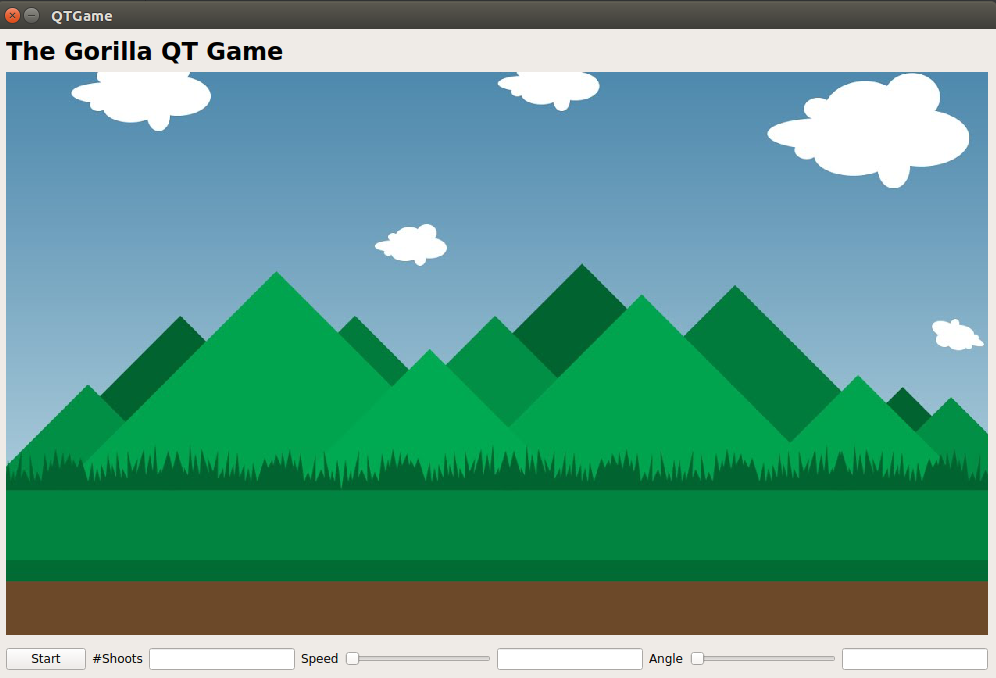
\includegraphics[width=220pt]{img/qtgamegui.png}
\end{frame}

\begin{frame}[fragile]
\frametitle{QT Game}
Gui Design - Class Diagram
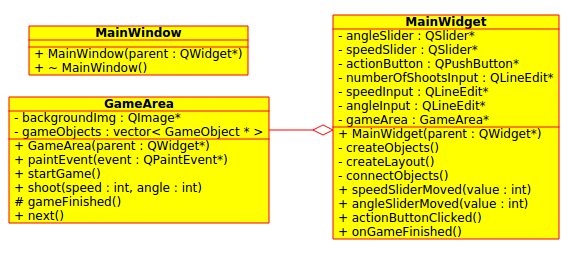
\includegraphics[width=220pt]{img/qtgame_cdgui.png}
\end{frame}

\begin{frame}[fragile]
\frametitle{QT Game}
Game Objects
\begin{itemize}
\item GameObject (abstract base class)
\item Player
\item Obstacle
\item Shoot
\end{itemize}
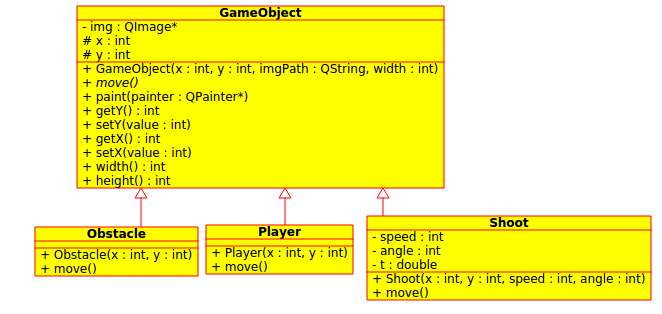
\includegraphics[width=220pt]{img/qtgame_cdgo.png}
\end{frame}

\begin{frame}[fragile]
\frametitle{QT Game}
Shoot - Projectile motion\\
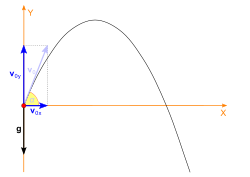
\includegraphics[width=100pt]{img/pro_motion.png}

{\small
\begin{lstlisting}
const double g = 9.81;
double rad = 3.1415926 / 180 * angle;
int dx = speed/3 * cos(rad) * t;
int dy = speed/3 * sin(rad) * t - (g/2) * pow(t,2);
t = t+0.1;
x = x + dx/2;
y = y - dy/2;
\end{lstlisting}
}
\end{frame}

\begin{frame}[fragile]
\frametitle{QT Game}
Thread
\begin{itemize}
\item Thread
\end{itemize}
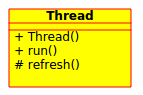
\includegraphics[width=100pt]{img/qtgame_cdthread.png}
\end{frame}

\begin{frame}[fragile]
\frametitle{QT Game}
Collision Detection
\begin{itemize}
\item CollisionDetection
\end{itemize}
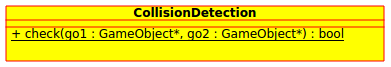
\includegraphics[width=220pt]{img/qtgame_cdcd.png}
\end{frame}

\begin{frame}[fragile]
\frametitle{QT Game}
Your additional tasks
\begin{itemize}
\item Rotating banana
\item Remove game objects if they are out of bounds
\item Include sound
\end{itemize}
\end{frame}


%\subsection{Database Access}
%\begin{frame}[fragile]
%\end{frame}
%\subsection{Network Connections}
%\begin{frame}[fragile]
%\end{frame}
